%% JSS manuscript — surveyframe: A Proactive Survey Research Workflow for R
%% Compile: pdflatex surveyframe && bibtex surveyframe && pdflatex surveyframe && pdflatex surveyframe

\documentclass[article]{jss}\usepackage[]{graphicx}\usepackage[]{xcolor}
% maxwidth is the original width if it is less than linewidth
% otherwise use linewidth (to make sure the graphics do not exceed the margin)
\makeatletter
\def\maxwidth{ %
  \ifdim\Gin@nat@width>\linewidth
    \linewidth
  \else
    \Gin@nat@width
  \fi
}
\makeatother

\definecolor{fgcolor}{rgb}{0.345, 0.345, 0.345}
\newcommand{\hlnum}[1]{\textcolor[rgb]{0.686,0.059,0.569}{#1}}%
\newcommand{\hlsng}[1]{\textcolor[rgb]{0.192,0.494,0.8}{#1}}%
\newcommand{\hlcom}[1]{\textcolor[rgb]{0.678,0.584,0.686}{\textit{#1}}}%
\newcommand{\hlopt}[1]{\textcolor[rgb]{0,0,0}{#1}}%
\newcommand{\hldef}[1]{\textcolor[rgb]{0.345,0.345,0.345}{#1}}%
\newcommand{\hlkwa}[1]{\textcolor[rgb]{0.161,0.373,0.58}{\textbf{#1}}}%
\newcommand{\hlkwb}[1]{\textcolor[rgb]{0.69,0.353,0.396}{#1}}%
\newcommand{\hlkwc}[1]{\textcolor[rgb]{0.333,0.667,0.333}{#1}}%
\newcommand{\hlkwd}[1]{\textcolor[rgb]{0.737,0.353,0.396}{\textbf{#1}}}%
\let\hlipl\hlkwb

\usepackage{framed}
\makeatletter
\newenvironment{kframe}{%
 \def\at@end@of@kframe{}%
 \ifinner\ifhmode%
  \def\at@end@of@kframe{\end{minipage}}%
  \begin{minipage}{\columnwidth}%
 \fi\fi%
 \def\FrameCommand##1{\hskip\@totalleftmargin \hskip-\fboxsep
 \colorbox{shadecolor}{##1}\hskip-\fboxsep
     % There is no \\@totalrightmargin, so:
     \hskip-\linewidth \hskip-\@totalleftmargin \hskip\columnwidth}%
 \MakeFramed {\advance\hsize-\width
   \@totalleftmargin\z@ \linewidth\hsize
   \@setminipage}}%
 {\par\unskip\endMakeFramed%
 \at@end@of@kframe}
\makeatother

\definecolor{shadecolor}{rgb}{.97, .97, .97}
\definecolor{messagecolor}{rgb}{0, 0, 0}
\definecolor{warningcolor}{rgb}{1, 0, 1}
\definecolor{errorcolor}{rgb}{1, 0, 0}
\newenvironment{knitrout}{}{} % an empty environment to be redefined in TeX

\usepackage{alltt}
\usepackage{amssymb}
\usepackage{orcidlink}

%% -- Author information -----------------------------------------------

\author{Mohammed Ali Sharafuddin~\orcidlink{0000-0001-5247-2964}\\Villa College, Maldives
   \And Meena Madhavan~\orcidlink{0000-0003-1244-5392}\\International Maritime College Oman}
\Plainauthor{Mohammed Ali Sharafuddin, Meena Madhavan}

\title{\pkg{surveyframe}: A Proactive Survey Research Workflow for \proglang{R}}
\Plaintitle{surveyframe: A Proactive Survey Research Workflow for R}
\Shorttitle{\pkg{surveyframe}: A Proactive Survey Research Workflow}

%% -- Abstract and keywords -----------------------------------------------

\Abstract{
Survey-based research in the social sciences, management, and health
disciplines typically follows a reactive pattern: an instrument is
built, data collected, and statistical techniques applied
retrospectively. This approach leaves the analysis plan unspecified
until after data collection, creating conditions for researcher degrees
of freedom, post-hoc model fitting, and irreproducible findings.

\pkg{surveyframe} introduces a \emph{proactive} workflow architecture
built around the \code{sframe} class, a typed, validated \proglang{R}
object that encodes the complete instrument specification, including
item definitions, response choice sets, scale membership, branching
logic, attention checks, and a pre-declared analysis plan, before a
single response is collected. Analysis is the execution of a
pre-declared methodological contract, not a search through analytical
space.

The package provides a constructor family for building \code{sframe}
instruments, SHA-256-integrity-checked serialisation to the
\code{.sframe} format, browser-based and \pkg{Shiny}-based survey
rendering, CSV-based and Google Sheets response collection, a
multi-stage quality-checking pipeline, scale scoring with reverse
coding, Cronbach's $\alpha$ and McDonald's $\omega$ reliability
statistics, EFA suitability diagnostics (KMO, Bartlett), lavaan CFA
syntax generation, a pre-declared analysis plan executor producing
APA-formatted results and interpretation prompts, and reproducible HTML
report generation. All core functions are available without optional
dependencies. Statistical extensions activate gracefully when
\pkg{psych} or \pkg{lavaan} are installed.

This article describes the design philosophy, the package architecture,
and demonstrates the complete workflow using a bundled tourism services
survey instrument and response dataset.
}

\Keywords{survey research, psychometrics, instrument design, reproducible research,
  \proglang{R}, pre-registration}
\Plainkeywords{survey research, psychometrics, instrument design, reproducible
  research, R, pre-registration}

%% -- Metadata (filled in by JSS on acceptance) ----------------------------
\Volume{VV}
\Issue{II}
\Month{MMMM}
\Year{YYYY}
\Submitdate{2026-06-17}
\Acceptdate{yyyy-mm-dd}

\Address{
  Mohammed Ali Sharafuddin\\
  Qasim Ibrahim School of Business\\
  Villa College, Mal\'{e} 20373, Maldives\\
  E-mail: \email{mohammed.ali@villacollege.edu.mv}\\
  ORCID: \href{https://orcid.org/0000-0001-5247-2964}{0000-0001-5247-2964}\\[1.5ex]
  Meena Madhavan\\
  Department of Logistics Management\\
  International Maritime College Oman (IMCO)\\
  National University of Science \& Technology\\
  Falaj Al Qabail, Sohar 322, Oman\\
  ORCID: \href{https://orcid.org/0000-0003-1244-5392}{0000-0003-1244-5392}
}

%% -------------------------------------------------------------------------
\IfFileExists{upquote.sty}{\usepackage{upquote}}{}
\begin{document}

%% -- Setup chunk (not shown in output) ------------------------------------



%% =========================================================================
\section{Introduction}
\label{sec:intro}
%% =========================================================================

Survey-based research is one of the most widely used methods across
the social sciences, management, education, and health disciplines.
A researcher designs an instrument, collects responses, and then
applies statistical procedures to the resulting data. In the dominant
tooling ecosystem (\proglang{SPSS} \citep{ibm2023}, SmartPLS
\citep{ringleetal2022}, \pkg{lavaan} \citep{rosseel2012}), the
statistical analysis is a distinct, post-hoc step performed after data
are in hand. The instrument, the analysis method, and the interpretation
criteria are often determined or refined only after examining the data.

This reactive pattern creates conditions that are now well-documented
in the reproducibility literature \citep{simmons2011, open2015}.
Researchers may, intentionally or not, adjust their scale definitions,
select among competing fit indices, or revise their theoretical model
after observing the data. Even when no scientific misconduct is
involved, the statistical consequences of such flexibility are severe:
inflated Type~I error rates, overfit models, and findings that do not
replicate \citep{gelman2014}.

Pre-registration disciplines the analysis plan by requiring researchers
to declare hypotheses, variables, and analysis procedures before data
collection \citep{nosek2018}. A growing number of journals and funders
now mandate or incentivise pre-registration. Yet most statistical
software provides no mechanisms to enforce or even express such a plan.
The analysis plan exists in a separate document, is manually followed,
and is never checked against the actual analysis executed.

\pkg{surveyframe} addresses this gap with a \emph{proactive workflow}
architecture. The central abstraction is the \code{sframe} class: a
typed \proglang{R} object that encodes the instrument definition
\emph{and} the intended analysis plan in a single, validated, and
integrity-checked object. The sframe is constructed before data
collection. The analysis is the execution of the plan embedded in the
instrument, not a new plan written after inspecting results. When a
researcher serialises an \code{sframe} to disk with \code{write\_sframe()},
an SHA-256 hash over the entire specification is stored alongside it.
If the instrument is later modified after data collection, the stored
hash provides an auditable record of the change.

This design is not a policy mechanism. Researchers can always construct
new analysis objects to run additional tests. What it provides is
\emph{visibility}: the pre-declared analysis is clearly separated from
any post-hoc exploration, making the distinction legible in both the
code and the final report.

\pkg{surveyframe} covers the complete survey research lifecycle:
instrument construction, validation, deployment as a self-contained
static HTML file or \pkg{Shiny} application, response collection and
import, data quality checking, scale scoring, reliability analysis,
EFA suitability diagnostics, lavaan CFA syntax generation, pre-declared
analysis plan execution, codebook generation, and HTML report rendering.
The package has three hard dependencies (\pkg{jsonlite}, \pkg{rlang},
\pkg{openssl}) and activates statistical extensions gracefully when
\pkg{psych} or \pkg{lavaan} are present.

The remainder of this article is organised as follows.
Section~\ref{sec:design} describes the design philosophy and the
\code{sframe} class.
Section~\ref{sec:construction} demonstrates instrument construction.
Section~\ref{sec:deployment} covers survey deployment and response
collection.
Section~\ref{sec:analysis} presents the analysis workflow.
Section~\ref{sec:reporting} describes reporting.
Section~\ref{sec:comparison} compares \pkg{surveyframe} with related
software.
Section~\ref{sec:summary} concludes.

%% =========================================================================
\section[Design philosophy and the sframe class]{Design philosophy and the \code{sframe} class}
\label{sec:design}
%% =========================================================================

\subsection{The proactive workflow}

The key architectural decision in \pkg{surveyframe} is that an
\code{sframe} object is always constructed from scratch, without data.
It describes an instrument and an intended analysis. Data are then
collected, imported, and passed into analysis functions alongside the
\code{sframe} as a second argument. The analysis functions read the
declared structure (scale membership, reverse coding, item types,
and analysis plan) from the instrument, not from the data.

This is in contrast to the typical \proglang{R} workflow in which a
researcher begins with a data frame and then constructs variable sets,
scale definitions, and model specifications interactively. In
\pkg{surveyframe}, those decisions must be made and committed to the
\code{sframe} before any data are in scope.

The practical consequence is that an sframe file produced before data
collection serves as a machine-readable proxy for a pre-registration.
When submitted to a pre-registration registry (e.g., OSF) alongside a
timestamp, or when used to derive the JSS replication file hash, the
\code{.sframe} file constitutes evidence that the analysis plan was
fixed before the results were observed.

\subsection[The sframe class]{The \code{sframe} class}

An \code{sframe} object is a named list with eight typed slots:

\begin{description}
  \item[\code{meta}] Character fields: \code{title}, \code{version},
    \code{description}, \code{authors}, \code{languages}, and
    \code{validated}.
  \item[\code{items}] A list of \code{sf\_item} objects, one per survey
    item.
  \item[\code{choices}] A list of \code{sf\_choices} objects, one per
    response scale.
  \item[\code{scales}] A list of \code{sf\_scale} objects defining
    composite scoring rules and measurement structure.
  \item[\code{branching}] A list of \code{sf\_branch} objects encoding
    conditional display logic.
  \item[\code{checks}] A list of \code{sf\_check} objects defining
    attention-check criteria.
  \item[\code{analysis\_plan}] A list of pre-declared analysis blocks,
    each specifying a test type, variable roles, and decision rules.
  \item[\code{models}] A list of \code{sf\_model} objects encoding
    structural relationships between constructs for CFA/SEM syntax
    generation.
\end{description}

The \code{sframe} is constructed via the \code{sf\_instrument()}
function, which accepts a \code{components} list of objects produced
by the \code{sf\_} constructor family. Components are sorted into their
respective slots automatically. Passing a non-constructor object raises
a validation error.

\subsection{Integrity and serialisation}

\code{write\_sframe()} serialises an \code{sframe} to the
\code{.sframe} format (a UTF-8 JSON container) and computes an
SHA-256 hash over the serialised content. The hash is stored in the
file header alongside the package version. \code{read\_sframe()}
recomputes the hash on load and aborts with a typed error of class
\code{sframe\_import\_error} if the stored and computed hashes differ,
indicating that the file was modified after serialisation. This
hash is the primary audit mechanism for detecting post-collection
instrument editing. The instrument hash is the first layer of a wider
proof-of-integrity framework for tamper-evident survey workflows
\citep{sharafuddin2026ssr}; later package versions extend hashing to
response data, analysis outputs, and a portable verification manifest.

%% =========================================================================
\section{Instrument construction}
\label{sec:construction}
%% =========================================================================

\subsection{Constructor family}

Six constructors produce the typed components assembled into an
\code{sframe}:

\begin{description}
  \item[\code{sf\_choices()}] Defines a named response scale (choice
    set) mapping numeric values to display labels. Choice sets are
    referenced by \code{id} in item definitions and reused across items
    sharing the same scale.
  \item[\code{sf\_item()}] Defines a single survey item. Supports
    thirteen item types: closed-response types
    (\code{"likert"}, \code{"single\_choice"}, \code{"multiple\_choice"},
    \code{"matrix"}, \code{"slider"}, \code{"ranking"}, \code{"rating"}),
    open-response types (\code{"numeric"}, \code{"text"},
    \code{"textarea"}, \code{"date"}), and layout elements
    (\code{"section\_break"}, \code{"text\_block"}).
  \item[\code{sf\_scale()}] Groups items into a composite scale and
    specifies scoring rules: \code{method} (\code{"mean"} or
    \code{"sum"}), \code{min\_valid} (minimum non-missing items for a
    valid score), \code{reverse\_items}, and optional item
    \code{weights}.
  \item[\code{sf\_branch()}] Defines a conditional display rule: an
    item is shown only when a specified condition on a prior item's
    response is met.
  \item[\code{sf\_check()}] Defines an attention-check criterion used
    by \code{quality\_report()} to flag inattentive respondents.
  \item[\code{sf\_model()}] Defines a measurement or structural model
    (\code{"efa"}, \code{"cfa"}, \code{"cb\_sem"}, or \code{"pls\_sem"})
    assembled from \code{sf\_construct()}, \code{sf\_path()},
    \code{sf\_covariance()}, and \code{sf\_indirect()} specifications.
    Declared models drive the CFA and SEM syntax generation described
    in Section~\ref{sec:analysis}.
\end{description}

\subsection{Building an instrument}

The following code constructs a minimal tourism services survey with
two constructs and five items, based on the instrument used throughout
the worked example in this article.

\begin{knitrout}
\definecolor{shadecolor}{rgb}{0.969, 0.969, 0.969}\color{fgcolor}\begin{kframe}
\begin{alltt}
\hlkwd{library}\hldef{(}\hlsng{"surveyframe"}\hldef{)}

\hlcom{## Define a shared 5-point agreement response scale}
\hldef{agree5} \hlkwb{<-} \hlkwd{sf_choices}\hldef{(}
  \hlkwc{id}     \hldef{=} \hlsng{"agree5"}\hldef{,}
  \hlkwc{values} \hldef{=} \hlnum{1}\hlopt{:}\hlnum{5}\hldef{,}
  \hlkwc{labels} \hldef{=} \hlkwd{c}\hldef{(}\hlsng{"Strongly disagree"}\hldef{,} \hlsng{"Disagree"}\hldef{,} \hlsng{"Neutral"}\hldef{,}
             \hlsng{"Agree"}\hldef{,} \hlsng{"Strongly agree"}\hldef{)}
\hldef{)}

\hlcom{## Define items: declare scale membership before any data exist}
\hldef{dm_1} \hlkwb{<-} \hlkwd{sf_item}\hldef{(}\hlsng{"dm_1"}\hldef{,}
  \hlsng{"Social media content influences my travel decisions."}\hldef{,}
  \hlkwc{type} \hldef{=} \hlsng{"likert"}\hldef{,} \hlkwc{choice_set} \hldef{=} \hlsng{"agree5"}\hldef{,}
  \hlkwc{scale_id} \hldef{=} \hlsng{"digital_marketing"}\hldef{,} \hlkwc{required} \hldef{=} \hlnum{TRUE}\hldef{)}

\hldef{dm_2} \hlkwb{<-} \hlkwd{sf_item}\hldef{(}\hlsng{"dm_2"}\hldef{,}
  \hlsng{"Online reviews shape my destination choices."}\hldef{,}
  \hlkwc{type} \hldef{=} \hlsng{"likert"}\hldef{,} \hlkwc{choice_set} \hldef{=} \hlsng{"agree5"}\hldef{,}
  \hlkwc{scale_id} \hldef{=} \hlsng{"digital_marketing"}\hldef{,} \hlkwc{required} \hldef{=} \hlnum{TRUE}\hldef{)}

\hldef{dm_3} \hlkwb{<-} \hlkwd{sf_item}\hldef{(}\hlsng{"dm_3"}\hldef{,}
  \hlsng{"Digital promotions encourage me to visit new places."}\hldef{,}
  \hlkwc{type} \hldef{=} \hlsng{"likert"}\hldef{,} \hlkwc{choice_set} \hldef{=} \hlsng{"agree5"}\hldef{,}
  \hlkwc{scale_id} \hldef{=} \hlsng{"digital_marketing"}\hldef{,} \hlkwc{required} \hldef{=} \hlnum{TRUE}\hldef{)}

\hldef{sq_1} \hlkwb{<-} \hlkwd{sf_item}\hldef{(}\hlsng{"sq_1"}\hldef{,}
  \hlsng{"The hospitality staff were attentive and helpful."}\hldef{,}
  \hlkwc{type} \hldef{=} \hlsng{"likert"}\hldef{,} \hlkwc{choice_set} \hldef{=} \hlsng{"agree5"}\hldef{,}
  \hlkwc{scale_id} \hldef{=} \hlsng{"service_quality"}\hldef{,} \hlkwc{required} \hldef{=} \hlnum{TRUE}\hldef{)}

\hldef{sq_2} \hlkwb{<-} \hlkwd{sf_item}\hldef{(}\hlsng{"sq_2"}\hldef{,}
  \hlsng{"Facilities were clean and well maintained."}\hldef{,}
  \hlkwc{type} \hldef{=} \hlsng{"likert"}\hldef{,} \hlkwc{choice_set} \hldef{=} \hlsng{"agree5"}\hldef{,}
  \hlkwc{scale_id} \hldef{=} \hlsng{"service_quality"}\hldef{,} \hlkwc{required} \hldef{=} \hlnum{TRUE}\hldef{)}

\hlcom{## Define scales — scoring rule committed before data collection}
\hldef{dm_scale} \hlkwb{<-} \hlkwd{sf_scale}\hldef{(}
  \hlkwc{id}     \hldef{=} \hlsng{"digital_marketing"}\hldef{,}
  \hlkwc{label}  \hldef{=} \hlsng{"Digital marketing effectiveness"}\hldef{,}
  \hlkwc{items}  \hldef{=} \hlkwd{c}\hldef{(}\hlsng{"dm_1"}\hldef{,} \hlsng{"dm_2"}\hldef{,} \hlsng{"dm_3"}\hldef{),}
  \hlkwc{method} \hldef{=} \hlsng{"mean"}
\hldef{)}

\hldef{sq_scale} \hlkwb{<-} \hlkwd{sf_scale}\hldef{(}
  \hlkwc{id}     \hldef{=} \hlsng{"service_quality"}\hldef{,}
  \hlkwc{label}  \hldef{=} \hlsng{"Service quality"}\hldef{,}
  \hlkwc{items}  \hldef{=} \hlkwd{c}\hldef{(}\hlsng{"sq_1"}\hldef{,} \hlsng{"sq_2"}\hldef{),}
  \hlkwc{method} \hldef{=} \hlsng{"mean"}
\hldef{)}

\hlcom{## Assemble the instrument}
\hldef{instr} \hlkwb{<-} \hlkwd{sf_instrument}\hldef{(}
  \hlkwc{title}       \hldef{=} \hlsng{"Tourism Experience Survey"}\hldef{,}
  \hlkwc{version}     \hldef{=} \hlsng{"1.0.0"}\hldef{,}
  \hlkwc{description} \hldef{=} \hlsng{"Digital marketing and service quality perceptions."}\hldef{,}
  \hlkwc{authors}     \hldef{=} \hlsng{"J. Researcher"}\hldef{,}
  \hlkwc{components}  \hldef{=} \hlkwd{list}\hldef{(agree5, dm_1, dm_2, dm_3, sq_1, sq_2,}
                     \hldef{dm_scale, sq_scale)}
\hldef{)}
\hlkwd{print}\hldef{(instr)}
\end{alltt}
\begin{verbatim}
## <sframe>
##   Title:      Tourism Experience Survey
##   Version:    1.0.0
##   Items:      5
##   Scales:     2
##   Status:     not validated
\end{verbatim}
\end{kframe}
\end{knitrout}

Each component class carries a small \proglang{S3} method surface, so the
constructor objects print and summarise cleanly at the console and inside
reports. The six component classes (\code{sf\_choices}, \code{sf\_item},
\code{sf\_scale}, \code{sf\_branch}, \code{sf\_check}, and \code{sf\_model})
each provide \code{print()}, \code{format()}, and \code{summary()} methods:

\begin{knitrout}
\definecolor{shadecolor}{rgb}{0.969, 0.969, 0.969}\color{fgcolor}\begin{kframe}
\begin{alltt}
\hlkwd{methods}\hldef{(}\hlkwc{class} \hldef{=} \hlsng{"sf_choices"}\hldef{)}
\end{alltt}
\begin{verbatim}
## [1] format  print   summary
## see '?methods' for accessing help and source code
\end{verbatim}
\end{kframe}
\end{knitrout}

\subsection{Validation}

\code{validate\_sframe()} checks the internal consistency of an
\code{sframe} object and reports all problems. The function performs
a battery of consistency checks, including duplicate item IDs, items
referencing missing choice sets, scale items not present in the
instrument, branching rules referencing unknown items, and analysis
plan roles referencing missing variables. In \code{strict = TRUE} mode
(the default), any problem raises a typed error of class
\code{sframe\_validation\_error}. In \code{strict = FALSE} mode, all
problems are returned as a character vector without stopping.

\begin{knitrout}
\definecolor{shadecolor}{rgb}{0.969, 0.969, 0.969}\color{fgcolor}\begin{kframe}
\begin{alltt}
\hldef{result} \hlkwb{<-} \hlkwd{validate_sframe}\hldef{(instr,} \hlkwc{strict} \hldef{=} \hlnum{FALSE}\hldef{)}
\hldef{result}\hlopt{$}\hldef{valid}
\end{alltt}
\begin{verbatim}
## [1] TRUE
\end{verbatim}
\begin{alltt}
\hldef{result}\hlopt{$}\hldef{problems}
\end{alltt}
\begin{verbatim}
## character(0)
\end{verbatim}
\end{kframe}
\end{knitrout}

\subsection{Serialisation}

\code{write\_sframe()} serialises a validated \code{sframe} to the
\code{.sframe} format and records an SHA-256 hash of the instrument
specification. The hash is computed over the canonical JSON
serialisation with the hash field itself set to an empty string, then
written into the file header. \code{read\_sframe()} recomputes the hash
on load and verifies it against the stored value:

\begin{knitrout}
\definecolor{shadecolor}{rgb}{0.969, 0.969, 0.969}\color{fgcolor}\begin{kframe}
\begin{alltt}
\hldef{path} \hlkwb{<-} \hlkwd{tempfile}\hldef{(}\hlkwc{fileext} \hldef{=} \hlsng{".sframe"}\hldef{)}
\hlkwd{write_sframe}\hldef{(instr, path)}

\hlcom{## The SHA-256 hash stored in the file header}
\hldef{stored_hash} \hlkwb{<-} \hldef{jsonlite}\hlopt{::}\hlkwd{fromJSON}\hldef{(path)}\hlopt{$}\hldef{hash}\hlopt{$}\hldef{value}
\hlkwd{substr}\hldef{(stored_hash,} \hlnum{1}\hldef{,} \hlnum{32}\hldef{)}
\end{alltt}
\begin{verbatim}
## [1] "7f06419e027d4f69b0a6e20c7c4342d8"
\end{verbatim}
\begin{alltt}
\hlcom{## read_sframe() recomputes and verifies the hash on load}
\hldef{instr2} \hlkwb{<-} \hlkwd{read_sframe}\hldef{(path)}
\hlkwd{identical}\hldef{(instr}\hlopt{$}\hldef{meta}\hlopt{$}\hldef{title, instr2}\hlopt{$}\hldef{meta}\hlopt{$}\hldef{title)}
\end{alltt}
\begin{verbatim}
## [1] TRUE
\end{verbatim}
\end{kframe}
\end{knitrout}

The hash verification on \code{read\_sframe()} detects out-of-band
modifications made after the file was created. Any change to the
serialised JSON, including edits to item text, scale membership, or
the analysis plan, produces a hash mismatch, and \code{read\_sframe()}
refuses to load the file, reporting both the expected and the stored
hash in the error message.

\subsection{Declaring the analysis plan}

An \code{sframe} optionally carries a pre-declared analysis plan as a
list of analysis blocks in the \code{analysis\_plan} slot. Blocks
specify the statistical test type, variable roles, options (e.g.,
$\alpha$ level), and decision rules. The bundled demonstration
instrument includes a full plan. The worked example in
Section~\ref{sec:analysis} runs it.

Analysis plans can be authored either programmatically or through the
visual SurveyBuilder interface described in
Section~\ref{sec:deployment}. When constructed through the interface,
the plan is stored in the \code{.sframe} file and retrieved by
\code{run\_analysis\_plan()} without any additional specification.

%% =========================================================================
\section{Survey deployment and response collection}
\label{sec:deployment}
%% =========================================================================

\subsection{Static HTML export}

\code{export\_static\_survey()} generates a self-contained single-file
HTML survey that runs entirely in the browser without a server or
internet connection. All thirteen item types, branching logic,
required-field validation, multi-page navigation, and progress
indication are implemented in client-side JavaScript. When a respondent
submits the form, the browser downloads a one-row CSV file. If an
\code{endpoint\_url} is supplied (a Google Apps Script web app or a
serverless function), the response is also POSTed as JSON. The CSV
download proceeds regardless of POST success, so no response is lost
on network failure.

A single call writes the deployable file. The instrument carries every
item, choice set, branching rule, and the page layout, so the export needs
no further arguments beyond the output path:

\begin{Code}
R> export_static_survey(instr,
+    output_path = "tourism_survey.html",
+    open = FALSE)
\end{Code}

The exported file can be hosted on any static file server, GitHub
Pages, Netlify, or sent as an email attachment. No server or R
installation is required on the respondent's machine.
Figures~\ref{fig:survey-welcome} to~\ref{fig:survey-mobile} show the
rendered survey from the bundled tourism instrument: the welcome screen,
a Likert item, the required-field validation message, and the mobile
layout. The same single HTML file produces all of these views.

%% Alt-text: A survey welcome page with the study title, a short
%% description, an estimated completion time, and a Start button.
\begin{figure}[t]
\centering
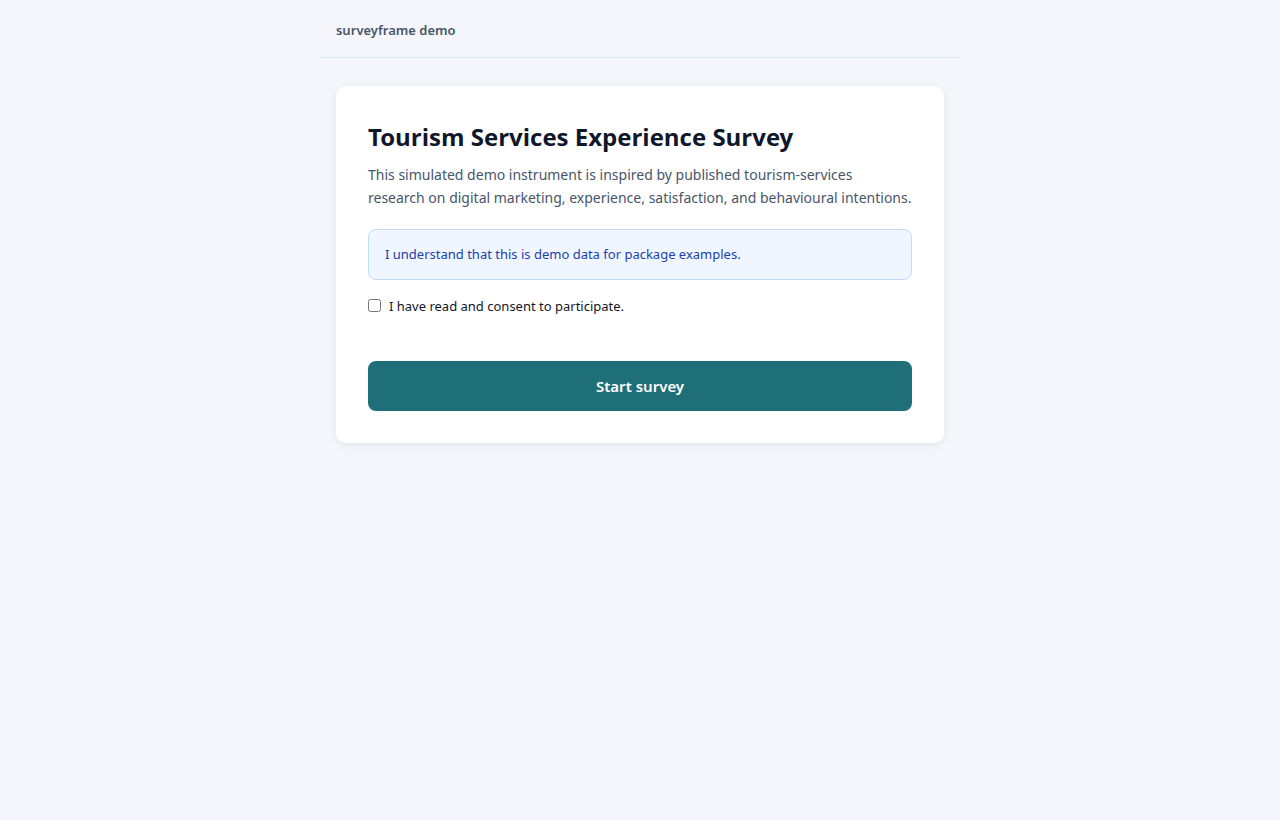
\includegraphics[width=0.62\textwidth]{figures/fig-survey-welcome.png}
\caption{The exported survey's welcome screen. It shows the instrument
  title, the description, an estimated completion time, and a Start
  button, rendered entirely in the browser from a single HTML file with
  no server.}
\label{fig:survey-welcome}
\end{figure}

%% Alt-text: A Likert survey question with a five-point agreement scale
%% and a progress bar near the top.
\begin{figure}[t]
\centering
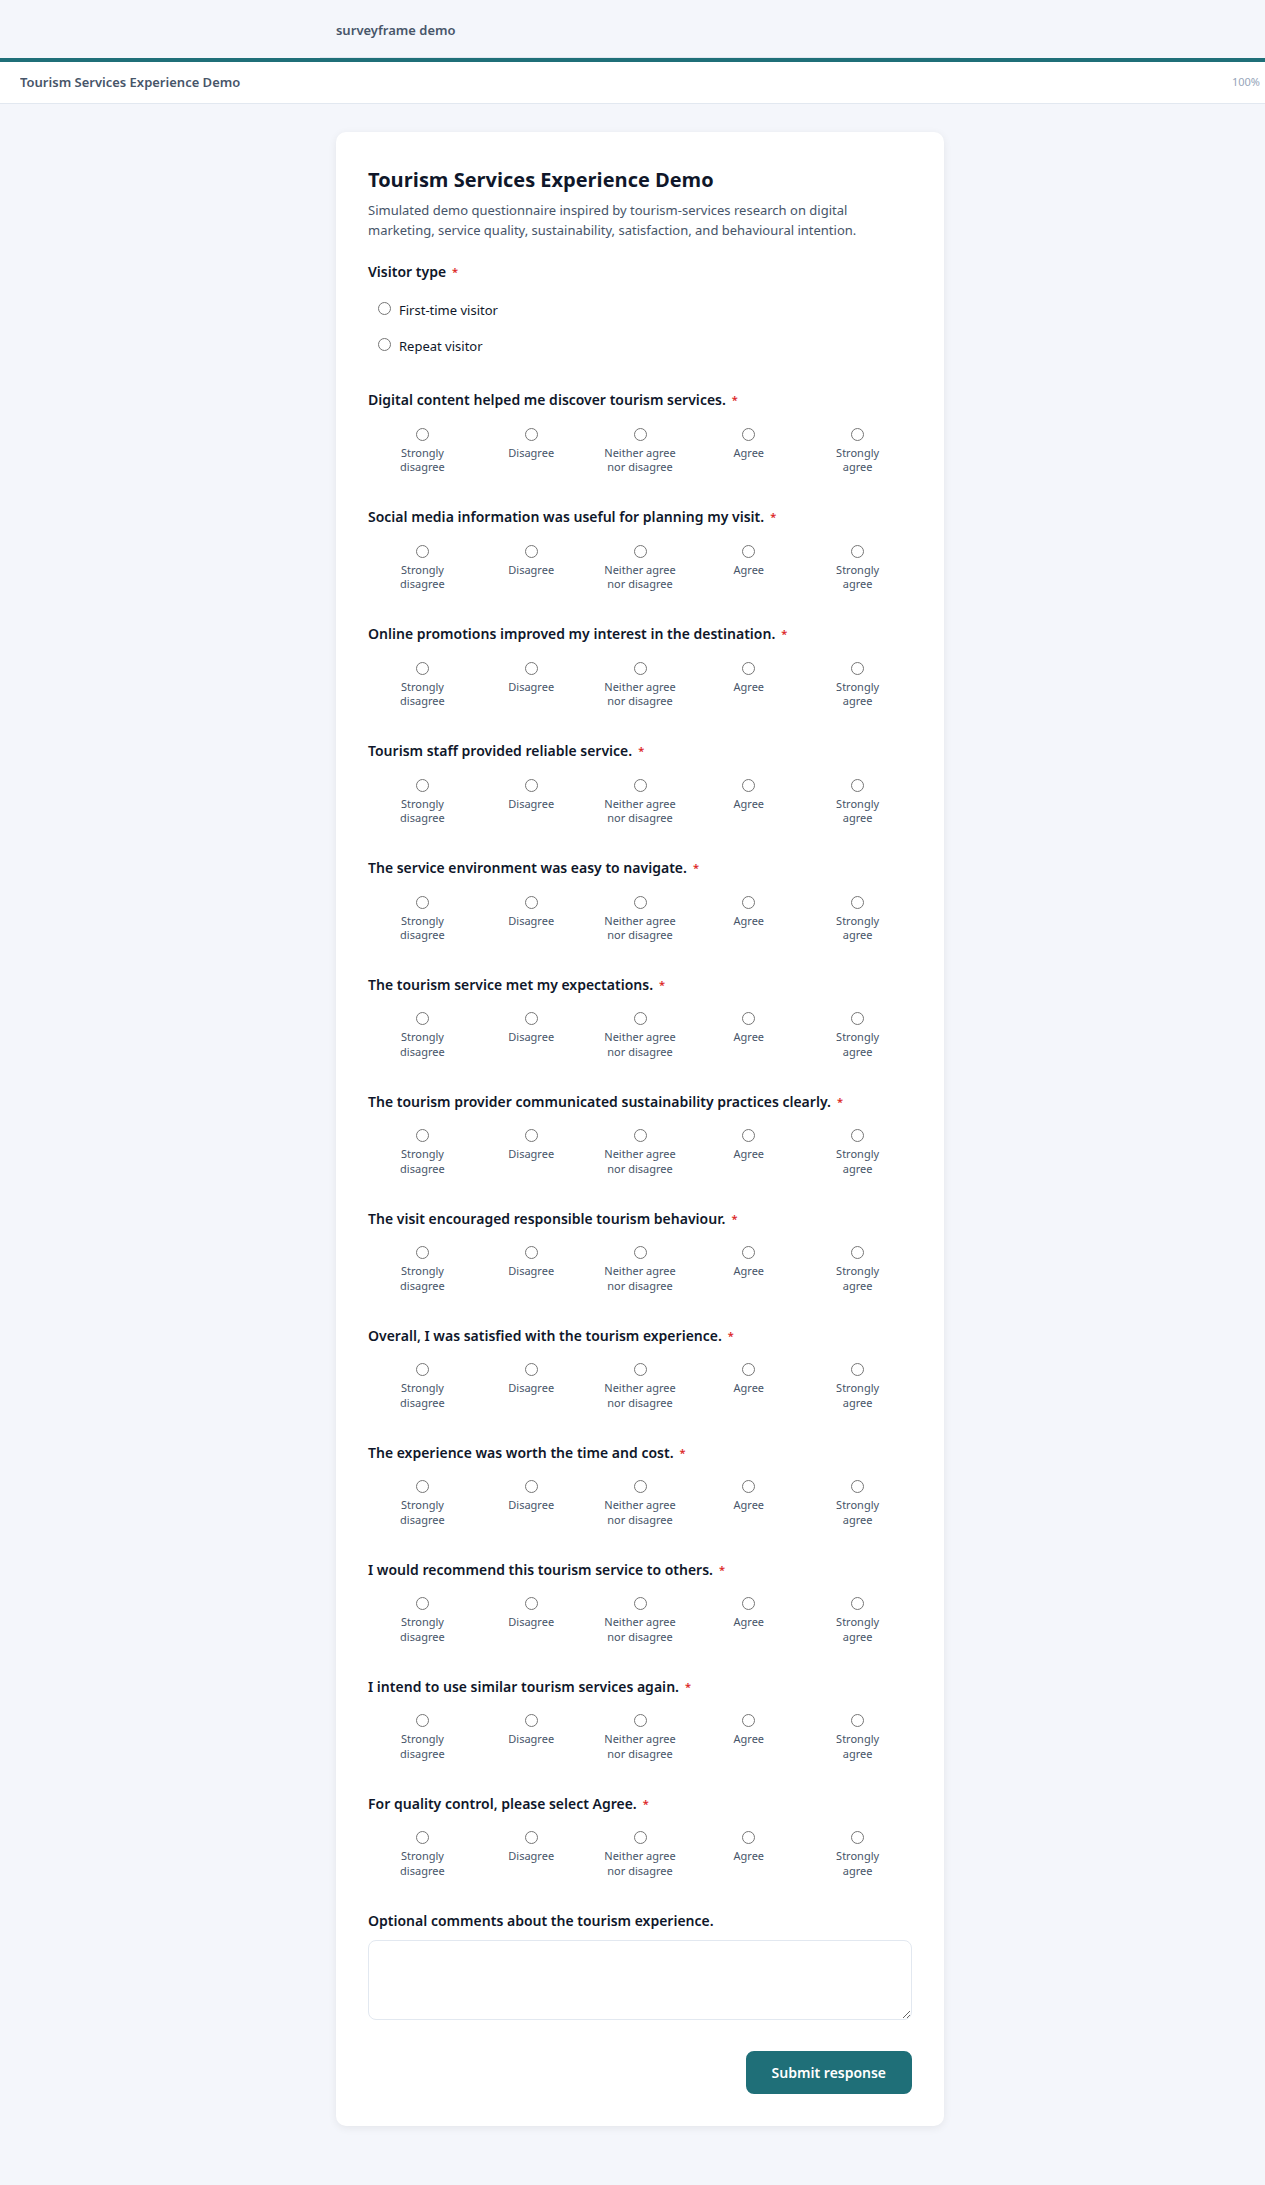
\includegraphics[width=0.62\textwidth]{figures/fig-survey-likert.png}
\caption{A five-point Likert item as rendered in the exported survey,
  with the page progress indicator above the question and the response
  options laid out for single selection.}
\label{fig:survey-likert}
\end{figure}

%% Alt-text: The same survey question showing a red inline validation
%% message because a required item was left unanswered.
\begin{figure}[t]
\centering
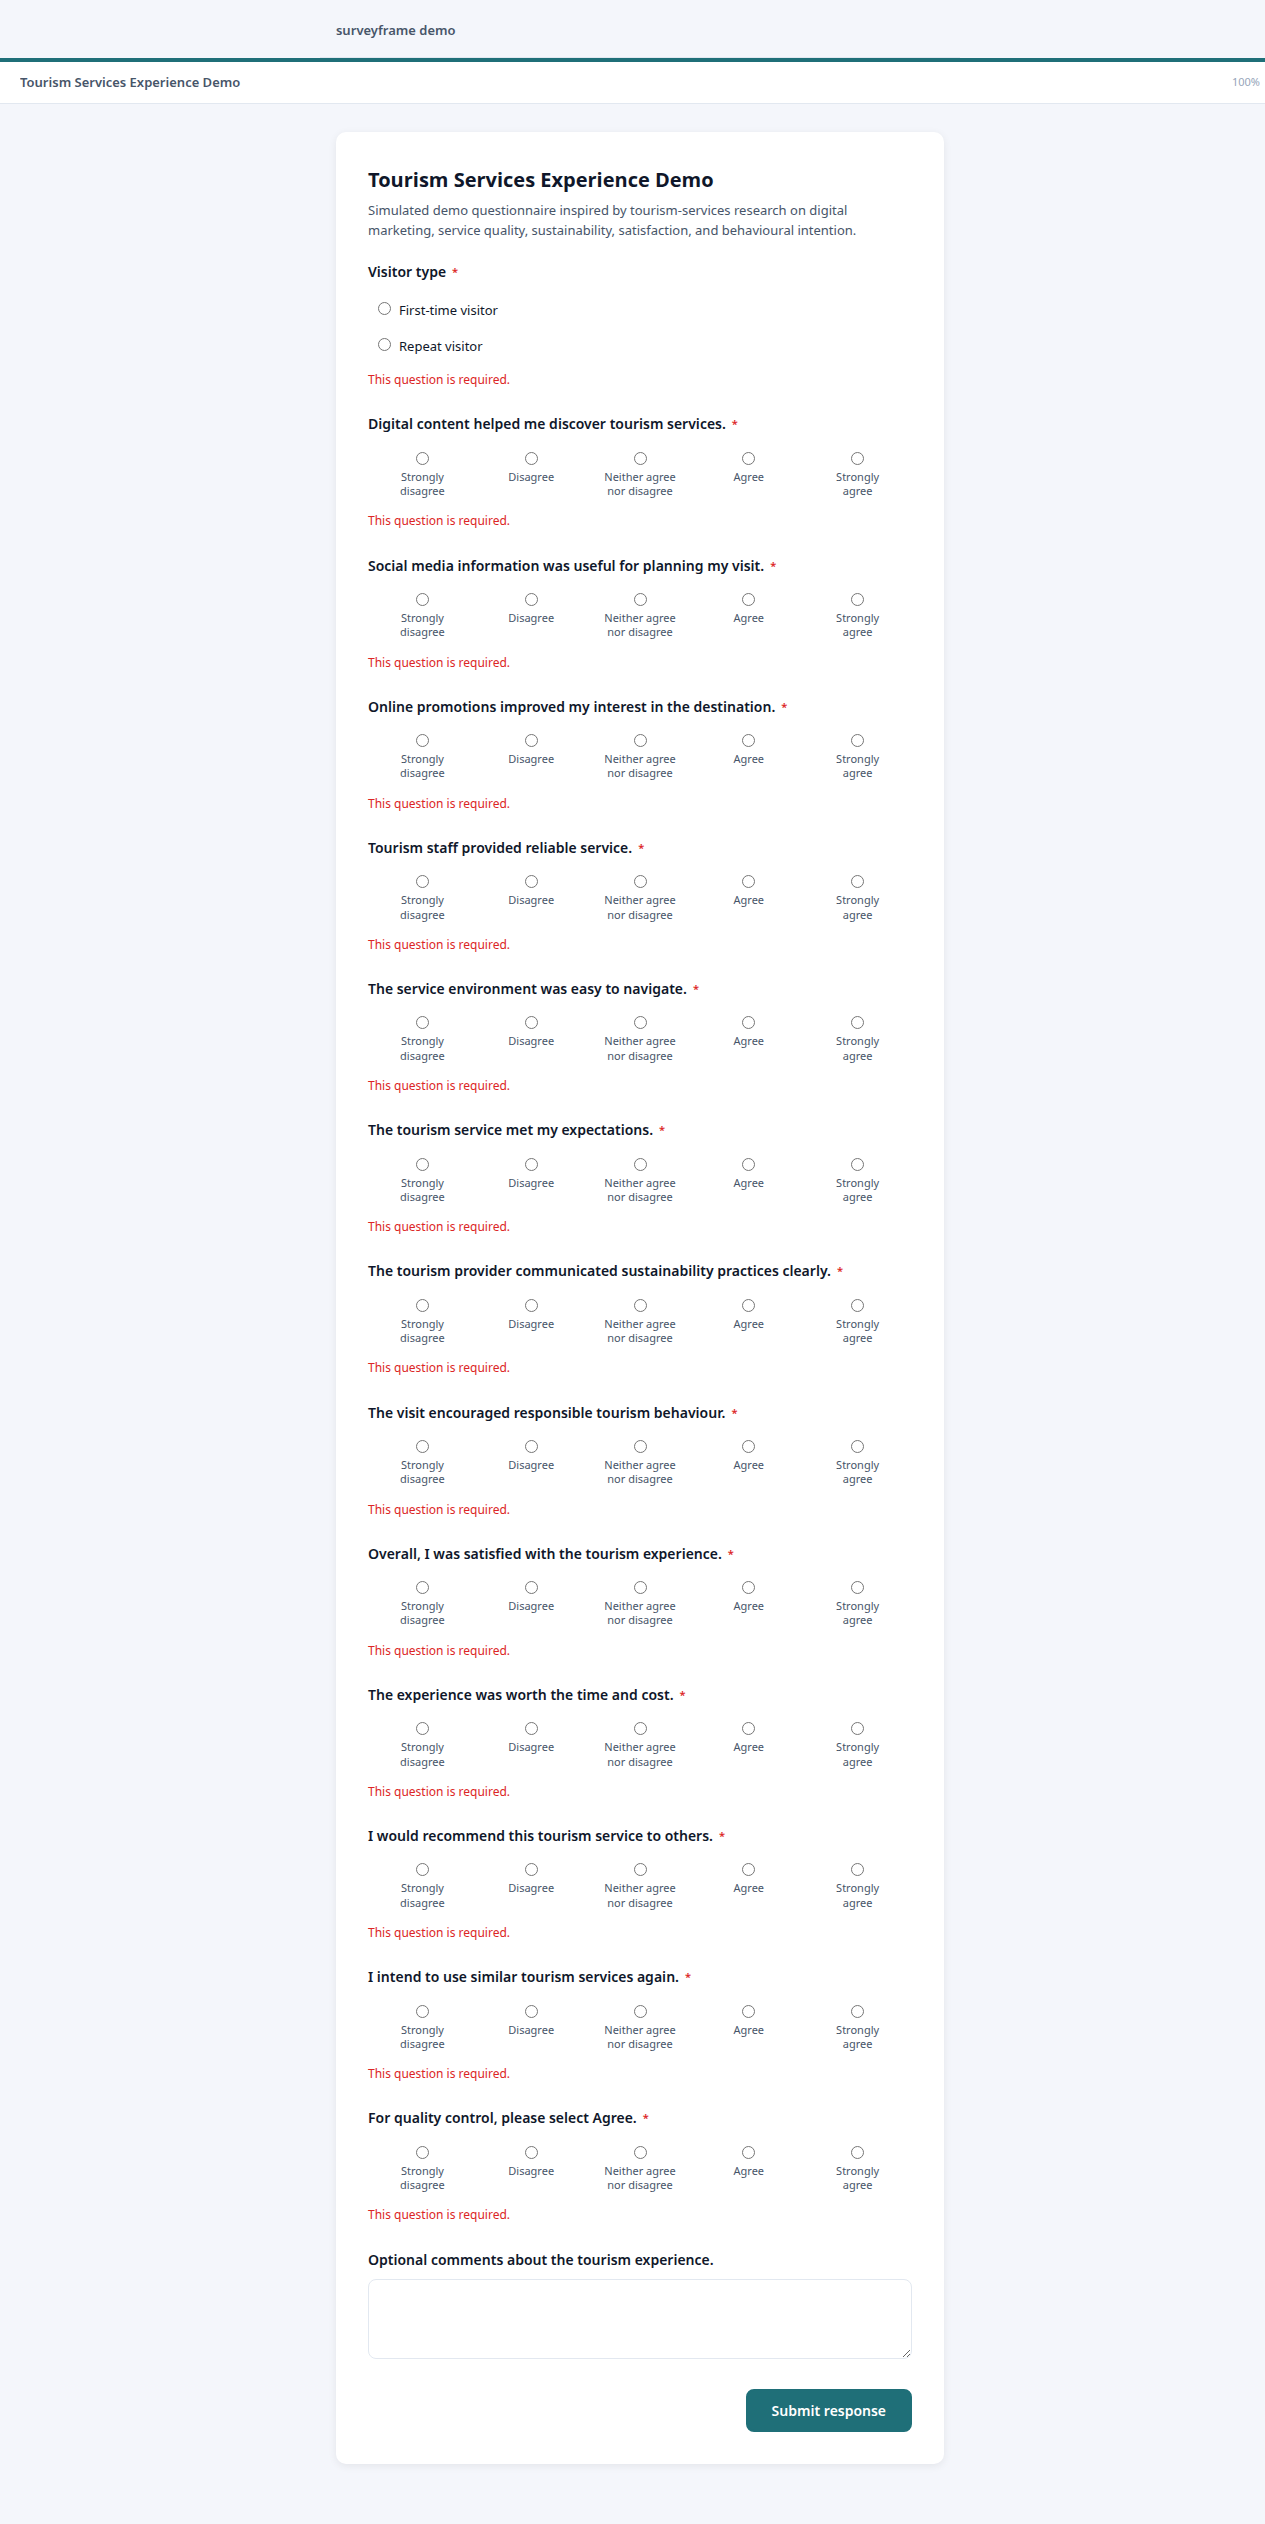
\includegraphics[width=0.62\textwidth]{figures/fig-survey-validation.png}
\caption{Client-side required-field validation. When a respondent tries
  to advance past a required item without answering, the survey blocks
  the move and shows an inline message, with no server round trip.}
\label{fig:survey-validation}
\end{figure}

%% Alt-text: The survey welcome screen rendered on a narrow phone-width
%% viewport, with the layout reflowed to a single column.
\begin{figure}[t]
\centering
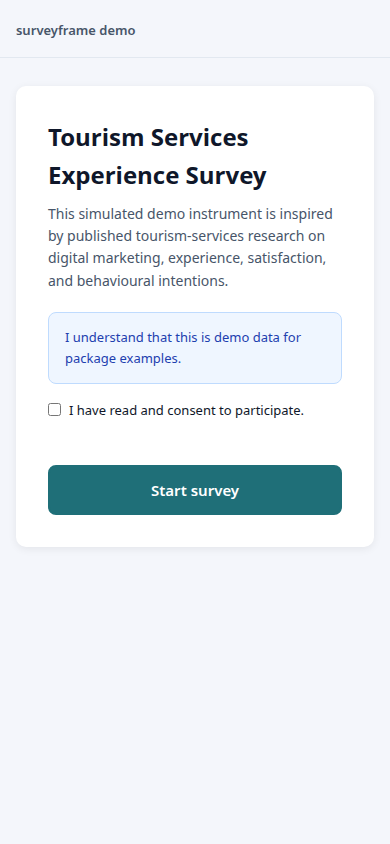
\includegraphics[width=0.32\textwidth]{figures/fig-survey-mobile.png}
\caption{The exported survey on a narrow, phone-width viewport. The
  layout reflows to a single column with touch-sized controls, so the
  same file serves desktop and mobile respondents.}
\label{fig:survey-mobile}
\end{figure}

\subsection{Visual SurveyBuilder}

\code{launch\_builder()} opens a browser-based visual instrument
editor. Researchers who prefer a graphical interface can build the
complete \code{sframe} (items, choice sets, scales, branching rules,
and analysis plan) without writing \proglang{R} code. The builder
exports the completed \code{.sframe} file. The file is imported into
\proglang{R} with \code{read\_sframe()} for analysis. The builder has
two modes: a Build mode for authoring items and scales
(Figure~\ref{fig:builder-build}) and an Analyse mode for declaring the
analysis plan and the measurement model (Figure~\ref{fig:builder-analyse}).

%% Alt-text: The SurveyBuilder Build mode, with an item list on the left,
%% an item editor in the centre, and instrument settings on the right.
\begin{figure}[t]
\centering
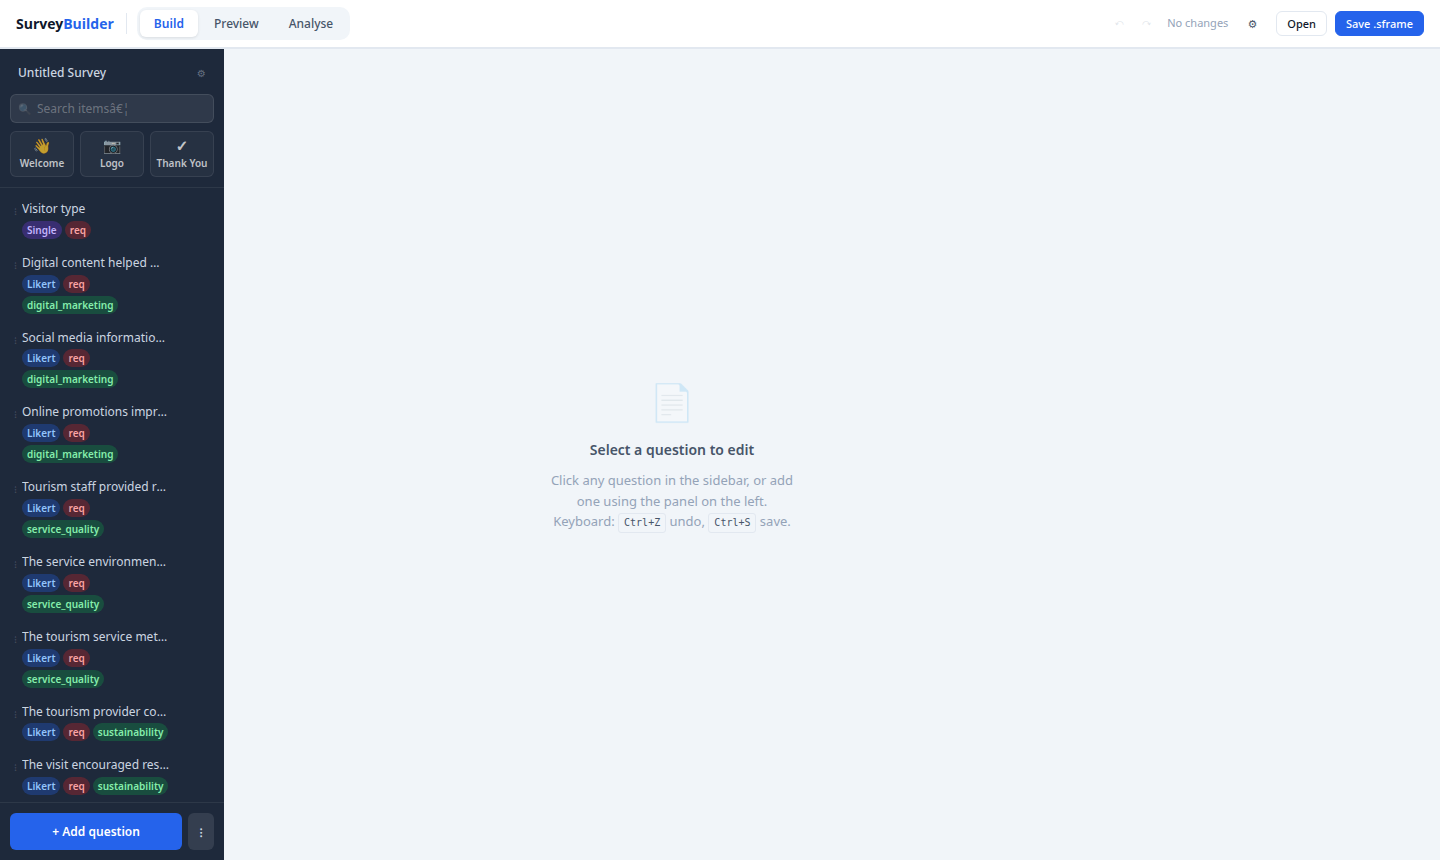
\includegraphics[width=0.9\textwidth]{figures/fig-builder-build.png}
\caption{SurveyBuilder Build mode. The left panel lists the items and
  scales, the centre edits the selected item and its response choices,
  and the right panel holds instrument settings. The builder runs in the
  browser and saves a \code{.sframe} file.}
\label{fig:builder-build}
\end{figure}

%% Alt-text: The SurveyBuilder Analyse mode, showing the analysis-plan
%% editor with research questions, methods, and variable roles.
\begin{figure}[t]
\centering
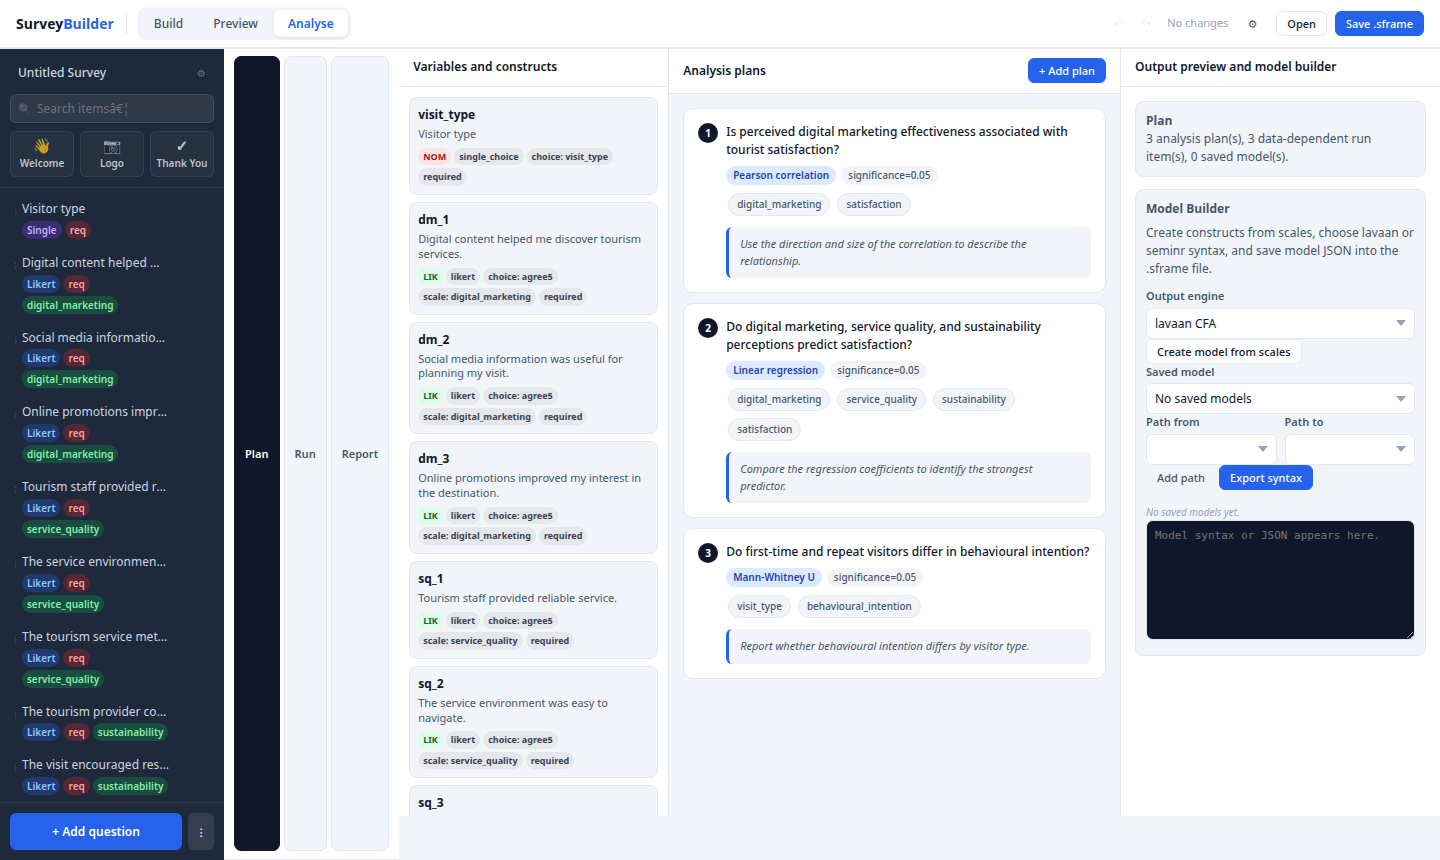
\includegraphics[width=0.9\textwidth]{figures/fig-builder-analyse.png}
\caption{SurveyBuilder Analyse mode. Each analysis block binds a research
  question to a statistical method and the variables that fill each role,
  and the measurement model is assembled alongside. The plan is stored in
  the \code{.sframe} file and executed later by
  \code{run\_analysis\_plan()}.}
\label{fig:builder-analyse}
\end{figure}

\subsection{Shiny survey module}

\code{render\_survey()} launches an interactive \pkg{Shiny} survey.
For embedding within a larger application, \code{survey\_module\_ui()}
provides the UI component and \code{survey\_module\_server()} provides
the server logic, returning a reactive that holds the response list
once the form is submitted.

\subsection{Response import}

\code{read\_responses()} reads a CSV file of responses, aligns item
columns against the instrument definition, and adds metadata columns
for respondent ID, submission timestamp, and any supplementary fields.
The function validates that all declared item columns are present and
warns if the column types are inconsistent with item definitions.

\begin{knitrout}
\definecolor{shadecolor}{rgb}{0.969, 0.969, 0.969}\color{fgcolor}\begin{kframe}
\begin{alltt}
\hldef{responses} \hlkwb{<-} \hlkwd{read_responses}\hldef{(}
  \hlkwc{x}             \hldef{=} \hlsng{"responses.csv"}\hldef{,}
  \hlkwc{instrument}    \hldef{= instr,}
  \hlkwc{respondent_id} \hldef{=} \hlsng{"respondent_id"}\hldef{,}
  \hlkwc{submitted_at}  \hldef{=} \hlsng{"submitted_at"}
\hldef{)}
\end{alltt}
\end{kframe}
\end{knitrout}

For the worked example that follows, the bundled demonstration dataset
is loaded directly:

\begin{knitrout}
\definecolor{shadecolor}{rgb}{0.969, 0.969, 0.969}\color{fgcolor}\begin{kframe}
\begin{alltt}
\hldef{demo}  \hlkwb{<-} \hlkwd{sframe_demo_data}\hldef{()}
\hldef{instr} \hlkwb{<-} \hldef{demo}\hlopt{$}\hldef{instrument}
\hldef{resp}  \hlkwb{<-} \hldef{demo}\hlopt{$}\hldef{responses}

\hlcom{## Five scales, 15 items, 120 respondents}
\hlkwd{cat}\hldef{(}\hlsng{"Scales:"}\hldef{,} \hlkwd{length}\hldef{(instr}\hlopt{$}\hldef{scales),} \hlsng{"\textbackslash{}n"}\hldef{)}
\end{alltt}
\begin{verbatim}
## Scales: 5
\end{verbatim}
\begin{alltt}
\hlkwd{cat}\hldef{(}\hlsng{"Items:"}\hldef{,} \hlkwd{length}\hldef{(instr}\hlopt{$}\hldef{items),} \hlsng{"\textbackslash{}n"}\hldef{)}
\end{alltt}
\begin{verbatim}
## Items: 15
\end{verbatim}
\begin{alltt}
\hlkwd{cat}\hldef{(}\hlsng{"Responses:"}\hldef{,} \hlkwd{nrow}\hldef{(resp),} \hlsng{"\textbackslash{}n"}\hldef{)}
\end{alltt}
\begin{verbatim}
## Responses: 120
\end{verbatim}
\end{kframe}
\end{knitrout}

%% =========================================================================
\section{The analysis workflow}
\label{sec:analysis}
%% =========================================================================

\pkg{surveyframe} structures the analysis workflow as a sequence of
discrete, composable steps. Each function accepts a data frame and an
\code{sframe} instrument as its primary arguments and returns a typed
object with a \code{print()} method. Steps can be executed
independently or as a complete pre-declared analysis plan.

\subsection{Data quality report}

\code{quality\_report()} performs five classes of quality checks on
the response data, using the instrument definition to determine what
constitutes a valid response:

\begin{enumerate}
  \item \textbf{Attention checks.} Flags respondents who fail declared
    \code{sf\_check()} criteria embedded in the instrument.
  \item \textbf{Timing.} When a start-time column is present, flags
    respondents who completed the survey faster than a declared
    minimum duration.
  \item \textbf{Straight-lining.} Flags respondents who gave the same
    response to every Likert item.
  \item \textbf{Missing data.} Reports per-item and per-respondent
    missingness rates.
  \item \textbf{Duplicates.} Detects duplicate respondent IDs.
\end{enumerate}

\begin{knitrout}
\definecolor{shadecolor}{rgb}{0.969, 0.969, 0.969}\color{fgcolor}\begin{kframe}
\begin{alltt}
\hldef{qr} \hlkwb{<-} \hlkwd{quality_report}\hldef{(resp, instr)}
\hlkwd{cat}\hldef{(}\hlsng{"Respondents:"}\hldef{, qr}\hlopt{$}\hldef{summary}\hlopt{$}\hldef{n_respondents,} \hlsng{"\textbackslash{}n"}\hldef{)}
\end{alltt}
\begin{verbatim}
## Respondents: 120
\end{verbatim}
\begin{alltt}
\hlkwd{cat}\hldef{(}\hlsng{"Items:      "}\hldef{, qr}\hlopt{$}\hldef{summary}\hlopt{$}\hldef{n_items,} \hlsng{"\textbackslash{}n"}\hldef{)}
\end{alltt}
\begin{verbatim}
## Items:       15
\end{verbatim}
\begin{alltt}
\hlkwd{cat}\hldef{(}\hlsng{"Flagged:    "}\hldef{, qr}\hlopt{$}\hldef{summary}\hlopt{$}\hldef{n_flagged,} \hlsng{"\textbackslash{}n"}\hldef{)}
\end{alltt}
\begin{verbatim}
## Flagged:     109
\end{verbatim}
\end{kframe}
\end{knitrout}

\subsection{Scale scoring}

\code{score\_scales()} computes composite scale scores for every
respondent according to the scoring rules declared in the
\code{sframe}. Reverse coding is applied automatically using either
the per-item \code{reverse} flag in \code{sf\_item()} or the
\code{reverse\_items} vector in \code{sf\_scale()}. Both sources are
respected. The \code{min\_valid} argument controls missingness
tolerance: respondents with fewer valid items than the declared
threshold receive \code{NA} for that scale.

\begin{knitrout}
\definecolor{shadecolor}{rgb}{0.969, 0.969, 0.969}\color{fgcolor}\begin{kframe}
\begin{alltt}
\hldef{scored} \hlkwb{<-} \hlkwd{score_scales}\hldef{(resp, instr)}
\hlcom{## Scale score columns appended to the response data frame}
\hldef{scale_cols} \hlkwb{<-} \hlkwd{c}\hldef{(}\hlsng{"digital_marketing"}\hldef{,} \hlsng{"service_quality"}\hldef{,}
                \hlsng{"sustainability"}\hldef{,} \hlsng{"satisfaction"}\hldef{,}
                \hlsng{"behavioural_intention"}\hldef{)}
\hlkwd{summary}\hldef{(scored[, scale_cols])}
\end{alltt}
\begin{verbatim}
##  digital_marketing service_quality sustainability  satisfaction 
##  Min.   :1.00      Min.   :1.33    Min.   :1.50   Min.   :1.00  
##  1st Qu.:2.67      1st Qu.:2.33    1st Qu.:2.50   1st Qu.:2.50  
##  Median :3.00      Median :3.00    Median :3.00   Median :3.25  
##  Mean   :3.15      Mean   :3.06    Mean   :3.19   Mean   :3.29  
##  3rd Qu.:3.67      3rd Qu.:3.67    3rd Qu.:4.00   3rd Qu.:4.00  
##  Max.   :5.00      Max.   :5.00    Max.   :5.00   Max.   :5.00  
##  behavioural_intention
##  Min.   :1.00         
##  1st Qu.:2.50         
##  Median :3.00         
##  Mean   :3.10         
##  3rd Qu.:3.62         
##  Max.   :5.00
\end{verbatim}
\end{kframe}
\end{knitrout}

\subsection{Reliability analysis}

\code{reliability\_report()} computes Cronbach's $\alpha$
\citep{cronbach1951} and McDonald's $\omega$ \citep{mcdonald1999} for
each scale in the instrument, using \pkg{psych} \citep{revelle2024}
when available. The function reads scale definitions directly from the
\code{sframe}, requiring no manual specification of item vectors.

\begin{knitrout}
\definecolor{shadecolor}{rgb}{0.969, 0.969, 0.969}\color{fgcolor}\begin{kframe}
\begin{alltt}
\hlkwa{if} \hldef{(}\hlkwd{requireNamespace}\hldef{(}\hlsng{"psych"}\hldef{,} \hlkwc{quietly} \hldef{=} \hlnum{TRUE}\hldef{)) \{}
  \hldef{rr} \hlkwb{<-} \hlkwd{reliability_report}\hldef{(resp, instr,} \hlkwc{omega} \hldef{=} \hlnum{FALSE}\hldef{)}
  \hlkwd{print}\hldef{(rr)}
\hldef{\}}
\end{alltt}
\begin{verbatim}
## Reliability Report
## 
## Scale: digital_marketing (Digital marketing effectiveness)
##   Items: 3   N: 120
##   Alpha:   0.837
## 
## Scale: service_quality (Service quality)
##   Items: 3   N: 120
##   Alpha:   0.844
## 
## Scale: sustainability (Sustainability perception)
##   Items: 2   N: 120
##   Alpha:   0.772
## 
## Scale: satisfaction (Tourist satisfaction)
##   Items: 2   N: 120
##   Alpha:   0.816
## 
## Scale: behavioural_intention (Behavioural intention)
##   Items: 2   N: 120
##   Alpha:   0.844
\end{verbatim}
\end{kframe}
\end{knitrout}

All five scales exceed the conventional $\alpha \geq 0.70$ threshold
\citep{nunnally1978}, supporting internal consistency.

\subsection{EFA suitability}

Before exploratory factor analysis, \pkg{surveyframe} evaluates
dataset suitability through the Kaiser-Meyer-Olkin (KMO) measure,
Bartlett's test of sphericity, and parallel analysis via
\code{efa\_report()}:

\begin{Code}
R> if (requireNamespace("psych", quietly = TRUE)) {
+    er <- efa_report(resp, instr)
+    print(er)
+  }
\end{Code}

The function constructs the item matrix from columns identified in the
instrument, passes it to \code{psych::KMO()},
\code{psych::cortest.bartlett()}, and \code{psych::fa.parallel()},
ensuring only the declared measurement items are included.

\subsection{CFA syntax generation}

\code{cfa\_syntax()} generates lavaan \citep{rosseel2012} CFA model
syntax directly from the scale definitions in the \code{sframe}. Each
scale becomes a reflective latent construct with its declared items as
indicators. The output is ready to pass to \code{lavaan::cfa()} when
\pkg{lavaan} is installed:

\begin{knitrout}
\definecolor{shadecolor}{rgb}{0.969, 0.969, 0.969}\color{fgcolor}\begin{kframe}
\begin{alltt}
\hldef{syn} \hlkwb{<-} \hlkwd{cfa_syntax}\hldef{(instr)}
\hlkwd{cat}\hldef{(syn)}
\end{alltt}
\begin{verbatim}
## # lavaan CFA syntax generated by surveyframe
## # Model: Tourism Services Experience Demo CFA
## # Recommended fitting option: std.lv = TRUE
## # Fit with lavaan only when lavaan is installed.
## 
## # Digital marketing effectiveness (reflective)
## digital_marketing =~ dm_1 + dm_2 + dm_3
## 
## # Service quality (reflective)
## service_quality =~ sq_1 + sq_2 + sq_3
## 
## # Sustainability perception (reflective)
## sustainability =~ sus_1 + sus_2
## 
## # Tourist satisfaction (reflective)
## satisfaction =~ sat_1 + sat_2
## 
## # Behavioural intention (reflective)
## behavioural_intention =~ bi_1 + bi_2
\end{verbatim}
\end{kframe}
\end{knitrout}

The syntax encodes the measurement model declared before data
collection. Because the construct-indicator relationships were
specified in \code{sf\_scale()} at instrument construction time, the
CFA tests a pre-declared structure rather than one selected after
inspecting inter-item correlations.

\subsection{Running the analysis plan}

\code{run\_analysis\_plan()} executes all analysis blocks declared in
the \code{sframe}'s \code{analysis\_plan} slot and returns an object
of class \code{sframe\_analysis\_results}. Each result carries the
test statistic, $p$~value, effect size, an APA-formatted summary
string, and a \code{prompt} field containing a plain-language interpretation
template that the researcher completes:

\begin{knitrout}
\definecolor{shadecolor}{rgb}{0.969, 0.969, 0.969}\color{fgcolor}\begin{kframe}
\begin{alltt}
\hldef{results} \hlkwb{<-} \hlkwd{run_analysis_plan}\hldef{(resp, instr,} \hlkwc{scored} \hldef{=} \hlnum{TRUE}\hldef{)}

\hlcom{## Correlation: digital marketing and satisfaction}
\hldef{r1} \hlkwb{<-} \hldef{results[[}\hlnum{1}\hldef{]]}
\hlkwd{cat}\hldef{(}\hlsng{"Test:  "}\hldef{, r1}\hlopt{$}\hldef{test,} \hlsng{"\textbackslash{}n"}\hldef{)}
\end{alltt}
\begin{verbatim}
## Test:   correlation_pearson
\end{verbatim}
\begin{alltt}
\hlkwd{cat}\hldef{(}\hlsng{"APA:   "}\hldef{, r1}\hlopt{$}\hldef{apa,} \hlsng{"\textbackslash{}n"}\hldef{)}
\end{alltt}
\begin{verbatim}
## APA:    r(118) = 0.54, p < .001
\end{verbatim}
\begin{alltt}
\hlkwd{cat}\hldef{(}\hlsng{"Effect:"}\hldef{, r1}\hlopt{$}\hldef{effect_label,} \hlsng{"\textbackslash{}n"}\hldef{)}
\end{alltt}
\begin{verbatim}
## Effect: large
\end{verbatim}
\begin{alltt}
\hlkwd{cat}\hldef{(}\hlsng{"Q:"}\hldef{,} \hlkwd{strwrap}\hldef{(r1}\hlopt{$}\hldef{research_question,} \hlkwc{width} \hldef{=} \hlnum{58}\hldef{,}
                  \hlkwc{exdent} \hldef{=} \hlnum{3}\hldef{),} \hlkwc{sep} \hldef{=} \hlsng{"\textbackslash{}n    "}\hldef{)}
\end{alltt}
\begin{verbatim}
## Q:
##     Is perceived digital marketing effectiveness associated
##        with tourist satisfaction?
\end{verbatim}
\begin{alltt}
\hlkwd{cat}\hldef{(}\hlsng{"\textbackslash{}n"}\hldef{)}
\end{alltt}
\end{kframe}
\end{knitrout}

The \code{prompt} field explicitly signals that the interpretation is
the researcher's responsibility: \pkg{surveyframe} provides the
statistic and its label. The researcher supplies the substantive
interpretation. This design discourages the conflation of statistical
and practical significance that is endemic in automated reporting tools.

The second analysis block in the bundled plan is a multiple regression:

\begin{knitrout}
\definecolor{shadecolor}{rgb}{0.969, 0.969, 0.969}\color{fgcolor}\begin{kframe}
\begin{alltt}
\hldef{r2} \hlkwb{<-} \hldef{results[[}\hlnum{2}\hldef{]]}
\hlkwd{cat}\hldef{(}\hlsng{"Test:"}\hldef{, r2}\hlopt{$}\hldef{test,} \hlsng{"\textbackslash{}n"}\hldef{)}
\end{alltt}
\begin{verbatim}
## Test: regression_linear
\end{verbatim}
\begin{alltt}
\hlkwd{cat}\hldef{(}\hlsng{"APA: "}\hldef{, r2}\hlopt{$}\hldef{apa,} \hlsng{"\textbackslash{}n"}\hldef{)}
\end{alltt}
\begin{verbatim}
## APA:  R² = 0.383, F(3, 116) = 23.95, p < .001
\end{verbatim}
\end{kframe}
\end{knitrout}

The third block tests whether first-time and repeat visitors differ in
behavioural intention using a Mann-Whitney $U$ test, appropriate
because \code{visit\_type} is a binary categorical predictor and
\code{behavioural\_intention} has a restricted range:

\begin{knitrout}
\definecolor{shadecolor}{rgb}{0.969, 0.969, 0.969}\color{fgcolor}\begin{kframe}
\begin{alltt}
\hldef{r3} \hlkwb{<-} \hldef{results[[}\hlnum{3}\hldef{]]}
\hlkwd{cat}\hldef{(}\hlsng{"Test:"}\hldef{, r3}\hlopt{$}\hldef{test,} \hlsng{"\textbackslash{}n"}\hldef{)}
\end{alltt}
\begin{verbatim}
## Test: mann_whitney
\end{verbatim}
\begin{alltt}
\hlkwd{cat}\hldef{(}\hlsng{"APA: "}\hldef{, r3}\hlopt{$}\hldef{apa,} \hlsng{"\textbackslash{}n"}\hldef{)}
\end{alltt}
\begin{verbatim}
## APA:  U = 1576, z = -0.98, p = 0.327, r = 0.09
\end{verbatim}
\begin{alltt}
\hlkwd{cat}\hldef{(}\hlsng{"Effect:"}\hldef{, r3}\hlopt{$}\hldef{effect_label,} \hlsng{"\textbackslash{}n"}\hldef{)}
\end{alltt}
\begin{verbatim}
## Effect: negligible
\end{verbatim}
\end{kframe}
\end{knitrout}

Supported analysis types include Pearson, Spearman, and Kendall
correlations, partial correlation, chi-square and Fisher's exact tests
of association, McNemar's test, Cochran's $Q$, independent and paired
$t$~tests, Mann-Whitney $U$, the Wilcoxon signed-rank test,
Kruskal-Wallis, Friedman's test, one-way and two-way ANOVA with Tukey
HSD, ANCOVA, repeated-measures ANOVA, linear regression, logistic
regression (binary, ordinal, and multinomial), mediation and moderation
templates, and descriptive, frequency, and missing-data blocks. Each
test type carries a curated citation list sourced from
the \code{.sframe\_citations} registry, providing the researcher with
the primary methodological references for their methods section.

%% =========================================================================
\section{Reporting}
\label{sec:reporting}
%% =========================================================================

\code{render\_report()} produces a self-contained HTML report
from the analysis results, instrument metadata, and codebook. The
report includes an executive summary, per-scale reliability statistics,
analysis plan results with APA-formatted tables, the full codebook,
and a citation block listing all packages and methodological references
used in the analysis. All output is contained in a single HTML file
that can be shared without external dependencies.

\begin{Code}
R> render_report(
+    instrument  = instr,
+    data        = resp,
+    output_file = "tourism_report.html"
+  )
\end{Code}

\code{codebook\_report()} generates a standalone codebook listing all
items, their types, choice sets, scale membership, and reverse-coding
status. The codebook can be exported as HTML or Markdown for inclusion
in supplementary materials or ethics board submissions.

\begin{knitrout}
\definecolor{shadecolor}{rgb}{0.969, 0.969, 0.969}\color{fgcolor}\begin{kframe}
\begin{alltt}
\hldef{cb} \hlkwb{<-} \hlkwd{codebook_report}\hldef{(instr)}
\hlkwd{nrow}\hldef{(cb}\hlopt{$}\hldef{items_table)}
\end{alltt}
\begin{verbatim}
## [1] 15
\end{verbatim}
\begin{alltt}
\hlkwd{head}\hldef{(cb}\hlopt{$}\hldef{items_table[,} \hlkwd{c}\hldef{(}\hlsng{"id"}\hldef{,} \hlsng{"type"}\hldef{,} \hlsng{"scale_id"}\hldef{,} \hlsng{"reverse"}\hldef{)],} \hlnum{6}\hldef{)}
\end{alltt}
\begin{verbatim}
##           id          type          scale_id reverse
## 1 visit_type single_choice                     FALSE
## 2       dm_1        likert digital_marketing   FALSE
## 3       dm_2        likert digital_marketing   FALSE
## 4       dm_3        likert digital_marketing   FALSE
## 5       sq_1        likert   service_quality   FALSE
## 6       sq_2        likert   service_quality   FALSE
\end{verbatim}
\end{kframe}
\end{knitrout}

The citation block in \code{render\_report()} automatically includes
citations for every test type run in the analysis plan, sourced from
the internal \code{.sframe\_citations} registry.

%% =========================================================================
\section{Comparison with existing software}
\label{sec:comparison}
%% =========================================================================

Table~\ref{tab:comparison} summarises \pkg{surveyframe} alongside the
principal existing tools for survey-based quantitative research.

\begin{table}[t]
\centering
\caption{Comparison of \pkg{surveyframe} with related software.
  \checkmark~= available, $\times$~= not available, P = planned.}
\label{tab:comparison}
\vspace{0.5em}
\footnotesize
\begin{tabular}{lcccccc}
\hline
Feature &
\pkg{survey\-frame} &
\proglang{SPSS} &
SmartPLS &
\pkg{lavaan} &
jamovi &
Qualtrics \\
\hline
Instrument construction     & \checkmark & \checkmark & $\times$ & $\times$ & $\times$ & \checkmark \\
Pre-declared analysis plan  & \checkmark & $\times$ & $\times$ & $\times$ & $\times$ & $\times$ \\
SHA-256 instrument hash     & \checkmark & $\times$ & $\times$ & $\times$ & $\times$ & $\times$ \\
Static HTML survey export   & \checkmark & $\times$ & $\times$ & $\times$ & $\times$ & $\times$ \\
Shiny survey module         & \checkmark & $\times$ & $\times$ & $\times$ & $\times$ & $\times$ \\
Scale scoring (mean/sum)    & \checkmark & \checkmark & \checkmark & $\times$ & \checkmark & $\times$ \\
Reliability ($\alpha$, $\omega$) & \checkmark & \checkmark & \checkmark & $\times$ & \checkmark & $\times$ \\
EFA suitability (KMO, Bartlett) & \checkmark & \checkmark & $\times$ & $\times$ & \checkmark & $\times$ \\
CFA syntax generation       & \checkmark & $\times$ & $\times$ & \checkmark & \checkmark & $\times$ \\
CB-SEM execution            & P & \checkmark & $\times$ & \checkmark & \checkmark & $\times$ \\
PLS-SEM execution           & P & $\times$ & \checkmark & $\times$ & $\times$ & $\times$ \\
APA results with citations  & \checkmark & $\times$ & $\times$ & $\times$ & $\times$ & $\times$ \\
HTML report generation      & \checkmark & $\times$ & $\times$ & $\times$ & \checkmark & \checkmark \\
CRAN open source            & \checkmark & $\times$ & $\times$ & \checkmark & \checkmark & $\times$ \\
Self-hostable               & \checkmark & $\times$ & $\times$ & \checkmark & \checkmark & $\times$ \\
No external calls           & \checkmark & \checkmark & \checkmark & \checkmark & \checkmark & $\times$ \\
\hline
\end{tabular}
\end{table}

\pkg{surveyframe}'s primary distinction is the \emph{proactive}
architecture: instrument construction, analysis plan declaration, and
data collection are strictly ordered. All other tools in
Table~\ref{tab:comparison} operate on data that already exist. None
require or provide mechanisms for encoding the analysis plan in the
instrument before data collection. This is the feature that most
directly addresses the reproducibility concerns outlined in
Section~\ref{sec:intro}.

\paragraph{SPSS.} SPSS \citep{ibm2023} is the GUI workhorse of much
social science and management research, with reliability analysis,
factor analysis, and regression long built in. It offers no
\proglang{R}-native scripting and no instrument-first workflow, and its
licence fees keep it out of reach for many individual researchers and
lower-income institutions.

\paragraph{SmartPLS.} SmartPLS \citep{ringleetal2022} is the popular
proprietary home of PLS-SEM, favoured in management research for
formative constructs and small samples. Everything happens inside its
own interface, with no \proglang{R} API and no way to declare the
instrument or the analysis plan up front. \pkg{surveyframe} already
writes \pkg{seminr} syntax for PLS-SEM, and fitting is on its roadmap.

\paragraph{lavaan.} \pkg{lavaan} \citep{rosseel2012} is the standard
\proglang{R} package for structural equation modelling, taking
researcher-written syntax and fitting it to a data frame.
\pkg{surveyframe} sits one step upstream: \code{cfa\_syntax()} writes
the lavaan measurement model straight from the \code{sframe} scales, so
the model that gets fitted is the one declared before any data arrived.

\paragraph{jamovi.} jamovi \citep{thejamoviproject2022} is a free,
open-source statistics GUI with an \proglang{R} API through \pkg{jmv},
covering descriptives, reliability, EFA, and CFA. It is the closest
match to the analysis and reporting end of \pkg{surveyframe}, though it
has no instrument design, static HTML export, or pre-declared analysis
plan.

%% =========================================================================
\section{Summary}
\label{sec:summary}
%% =========================================================================

\pkg{surveyframe} introduces a proactive architecture for survey-based
research in \proglang{R}. The \code{sframe} class encodes the complete
research instrument (items, response scales, composite scale
definitions, branching logic, and analysis plan) in a single validated
and integrity-checked object constructed before data collection. This
design makes the distinction between a pre-declared analysis and
post-hoc exploration explicit in the code and the final report,
directly supporting the methodological standards demanded by
reproducible-research initiatives and pre-registration mandates.

The package covers the complete survey research lifecycle: instrument
construction and validation, SHA-256-integrity-checked serialisation,
browser-based and Shiny-based survey rendering, static HTML export for
offline or server-free deployment, CSV and Google Sheets response
collection, a multi-stage data quality pipeline, scale scoring with
automatic reverse coding, Cronbach's $\alpha$ and McDonald's $\omega$
reliability statistics, EFA suitability diagnostics, lavaan CFA syntax
generation, a pre-declared analysis plan executor with APA-formatted
results and interpretation prompts, codebook generation, and HTML
report rendering.

\pkg{surveyframe} v0.3.2 is available on CRAN. Planned extensions
include PLS-SEM and CB-SEM execution via \pkg{seminr} and \pkg{lavaan},
item response theory workflows, multi-criteria decision making,
Quarto-native report generation, and the remaining layers of the
proof-of-integrity framework \citep{sharafuddin2026ssr}, which extend
the instrument hash to response data, analysis outputs, and a portable
verification manifest. The package repository and issue
tracker are available at
\url{https://github.com/MohammedAliSharafuddin/surveyframe}.

%% =========================================================================
%% References
%% =========================================================================

\bibliography{surveyframe}

%% =========================================================================
%% Session information
%% =========================================================================

\begin{appendix}

\section{Session information}
\label{app:session}

\begin{kframe}
\begin{alltt}
\hlkwd{toLatex}\hldef{(}\hlkwd{sessionInfo}\hldef{())}
\end{alltt}
\end{kframe}\begin{itemize}\raggedright
  \item R version 4.6.0 (2026-04-24), \verb|x86_64-pc-linux-gnu|
  \item Locale: \verb|LC_CTYPE=en_GB.UTF-8|, \verb|LC_NUMERIC=C|, \verb|LC_TIME=en_IN.UTF-8|, \verb|LC_COLLATE=en_GB.UTF-8|, \verb|LC_MONETARY=en_IN.UTF-8|, \verb|LC_MESSAGES=en_GB.UTF-8|, \verb|LC_PAPER=en_IN.UTF-8|, \verb|LC_NAME=C|, \verb|LC_ADDRESS=C|, \verb|LC_TELEPHONE=C|, \verb|LC_MEASUREMENT=en_IN.UTF-8|, \verb|LC_IDENTIFICATION=C|
  \item Time zone: \verb|Indian/Maldives|
  \item TZcode source: \verb|system (glibc)|
  \item Running under: \verb|Ubuntu 26.04 LTS|
  \item Matrix products: default
  \item BLAS:   \verb|/usr/lib/x86_64-linux-gnu/blas/libblas.so.3.12.1|
  \item LAPACK: \verb|/usr/lib/x86_64-linux-gnu/lapack/liblapack.so.3.12.1|
; \quad\ LAPACK version3.12.0
  \item Base packages: base, datasets, graphics,
    grDevices, methods, stats, utils
  \item Other packages: surveyframe~0.3.2
  \item Loaded via a namespace (and not attached):
    askpass~1.2.1, cli~3.6.6, compiler~4.6.0,
    evaluate~1.0.5, GPArotation~2026.4-1, grid~4.6.0,
    highr~0.12, jsonlite~2.0.0, knitr~1.51,
    lattice~0.22-9, MASS~7.3-65, mnormt~2.1.2,
    nlme~3.1-169, openssl~2.4.2, otel~0.2.0,
    parallel~4.6.0, psych~2.6.5, rlang~1.2.0,
    stats4~4.6.0, tools~4.6.0, xfun~0.58
\end{itemize}


\section{Replication}

All results in this manuscript are reproducible using the
\code{replicate.R} script included with the submission. The script
loads \pkg{surveyframe}, calls \code{sframe\_demo\_data()} to obtain
the bundled instrument and response dataset, and executes every code
example shown above in sequence. No additional data files or network
access are required.

\end{appendix}

\end{document}
